\chapter{Analysis}
\section{Introduction}
Consider in how many ways can we arrange the set $\{1,2,3\}$: 
\[
\{1, 2, 3\}, \{1, 3, 2\}, \{2, 1, 3\}, \{2, 3, 1\}, \{3, 1, 2\}, \{3, 2, 1\}
\]
that is we have $3$ ways of choosing the first element, and $3-1$ options for the second
(as we cannot repeat the first choise) and $3-2$ for the last (as non of the former two choices may be used),
therefor we can arrange them in $3 \cdot 2 \cdot 1 = 6$ ways. In general we define the number of 
permutations of a set with $n$ elements as the faculty function $n!$
\[
n! = n \cdot (n-1) \cdot (n-2) \cdots  (n - (n -1)) = 1 \cdot 2 \cdots n = \prod_{k=1}^{n}k, 
\]

the last notation is new but simply means that we multiply all the values of $k$ from $1$
to $n$. A recursive version (a self-calling function) can be constructed by noting that $n! =
n(n-1)!$. \\

\myindent Now consider a slightly more complex question: in how many ways can we pick two 
elements from the set $\{1,2,3\}$, the answer turns out to be three ways: 
\[
\{1, 2\}, \{1, 3\}, \{2, 3\}
\]
To generalize this we can ask in how many ways can we pick a unordered subset with $k$ elements from a set with $n$
elements ?. To answer this, observe there are $n$ choices for the first element and for each of these there are 
$n - 1$ choices for the second; and so on until there are $n - k + 1$ for the k'th and thus $n(n-1) \cdots (n - k + 1)$ 
choices for picking a $k$-element sequence from $n$. Now since each $k$-element subset has exactly $k!$ different 
orderings, we get our answer by dividing with $k!$:
\begin{equation}\label{binom}
\binom{n}{k} = \frac{n(n-1) \cdots (n - k + 1)}{k!},  \qquad \text{integer } n \geq k \geq 0
\end{equation}
and if we multiply the numerator and denominator of \ref{binom} by $(n - k)!$ we get:
\[
\frac{n(n-1) \cdots (n - k + 1)}{k!} \cdot \frac{(n - k)!}{(n - k)!} =  \frac{n!}{k!(n-k)!}
\]
The symbol $\binom{n}{k}$ is known as a binomial coefficient and we read it "$n$ choose $k$". Using this result we can
calculating the above question about choosing two elements from a three element set as:
\[
\binom{3}{2}  = \frac{3!}{2! (3-2)!} = \frac{3 \cdot 2 \cdot 1}{2 \cdot 1 \cdot 1} = 3
\]
Interestingly when determining the number of ways to pick $k$ elements we have in effect also specified the $n-k$
unchosen things, therefore 
\begin{equation}\label{binom_symmetry}
\binom{n}{k} = \binom{n}{n-k} 
\end{equation}
this symmetry can be observed in the above example where we have $3$ ways of picking $2$ elements from a $3$-element set
but then also $3$ ways of picking the remaining element. It also follows directly from the definition of the binomial
coefficient 
\[
\binom{n}{k} =  \frac{n!}{k!(n-k)!} =  \frac{n!}{(n-(n-k))!(n-k)!} = \binom{n}{n-k}
\]

\myindent Another rather remarkable result, known as Pascal's rule, can be derived by marking a particular object
$\epsilon$ in an $n$-element set. Now if we pick $k$ objects from $n$, then either $\epsilon$ is picked or it is not. If
$\epsilon$ is in the subset then there is $k-1$ objects left to choose among the $n-1$ elements, or more formally
$\binom{n-1}{k-1}$. If $\epsilon$ is not in the subset, we need to choose all the $k$ elements in the subset from the
$n-1$ objects that are not $\epsilon$; formally that is $\binom{n-1}{k}$. Thus there are 
\[
\binom{n-1}{k-1} + \binom{n-1}{k}
\]
ways to choose $k$ elements from $n$ depending on whether $\epsilon$ is included in each selection or not. But this
number must be the same as the binomial coefficient and thus we get: 
\begin{equation}\label{pascal_rule}
\binom{n}{k}  = \binom{n-1}{k-1} + \binom{n-1}{k}
\end{equation}
Those who consider the above reasoning a bit vague may rejoice from the following straightforward algebraic manipulation
\begin{align*}
 \binom{n-1}{k-1} + \binom{n-1}{k} 
& =  \frac{(n-1)!}{(k-1)!((n-1)-(k-1))!} + \frac{(n-1)!}{k!((n - 1) - k)!} \\
& =  \frac{(n-1)!}{(k-1)!(n-k)!} + \frac{(n-1)!}{k!(n - (k + 1))!} \\
& =  \frac{k(n-1)!}{k!(n-k)!} + \frac{(n-1)!(n-k)}{k!(n - k)!} \\
& =  \frac{(n-1)!(k + n - k)}{k!(n-k)!} \\
& =  \frac{n!}{k!(n-k)!} 
\end{align*}
It is interesting to notice that in the field of combinatorics we can arrive at the same result in different ways.
Indeed the smart mathematician should always seek alternate routes whenever a result causes the least headache.

%% CAPSULE
\begin{framed}
\begin{wrapfigure}{r}{0pt}
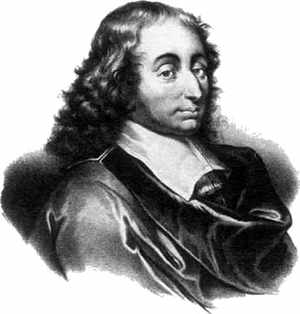
\includegraphics[width=4cm]{images/blaise_pascal.jpg}
\end{wrapfigure} 
\textbf{Blaise Pascal} ($1623-1662$)\\ French mathematician, physicist, and religious philosopher. He
was a child prodigy who already at the age of sixteen was corresponding, by letter, with the mighty Rene Descartes
($1596-1650$). When Descartes later leaned the age of Pascal he refused to believe that so young a boy was the author of
such brilliant mathematics. 

\myindent Pascal, like Newton, was a devoted theologist who spend most of his life pondering religious questions instead
of mathematical ones. By studying omens in the events around him he in fact ended up dropping mathematics completely,
since he found it apparent that God's plan for him did not include mathematics. But at the age of $35$ Pascal observed
that a particular nagging toothache seamed to go away when he pondered about mathematical things.  He concluded that
this was a good omen and thus spend one week in hectic mathematical activity. He never returned to mathematics after
this and died at the age of 39. 

\myindent Even with such a short and unfocused scientific career, Pascal managed to do become a first rate scientist. He
made important contributions to the construction of mechanical calculators, the study of fluids, and clarified the
concepts of pressure and vacuum. Pascal also helped create two major new areas of research. He wrote a significant
treatise on the subject of projective geometry and later corresponded with Pierre de Fermat on probability theory.
\end{framed}


%% PASCALs TRIANGLE
\myindent From Pascal's rule we can construct his famous triangle. Observe that according to this rule (see \ref{pascal_rule}) you can calculate $\binom{5}{3}$ as:
\begin{align*}
 \binom{5}{3}
& =  \binom{4}{3} + \binom{4}{2}  \\
& =  \binom{4}{3} + \binom{3}{2} +  \binom{3}{1} \\
& =  \binom{4}{3} + \binom{3}{2} +  \binom{2}{1} + \binom{2}{0} \\
\end{align*}
as $\binom{2}{0} = 1$, we can stop the expansion. In general as $\binom{n}{n}$ and $\binom{n}{0}$ are always
$1$ (when $n \geq 0$) we are guarantied that the expansion always terminates. Thus we have found a convenient way of
expressing higher binomial coefficients as sums of consecutive smaller ones:\\ 
\begin{center}
\begin{tabular}{l|*{5}{c}r}
\toprule
$n$ & $\binom{n}{0}$        & $\binom{n}{1}$ & $\binom{n}{2}$ & $\binom{n}{3}$ & $\binom{n}{4}$  & $\binom{n}{5}$ \\
\hline
0		& 1                     & 0 			       & 0 			        & 0 			       & 0 			         & 0   \\
1   & 1                     & 1 			       & 0 			        & 0 			       & 0  			       & 0   \\
2   & 1                     & 2 			       & 1 			        & 0 			       & 0  			       & 0   \\
3		& 1                     & 3 			       & 3 			        & 1			         & 0  			       & 0   \\
4		& 1                     & 4 			       & 6 			        & 4			         & 1  			       & 0   \\
5		& 1                     & 5 			       & 10 			      & 10			       & 5  			       & 1   \\
\bottomrule
\end{tabular}
\end{center}
discarding the zero's we can arrange these numbers into a triangle: 
\[
\begin{array}{c} 
1 \\ 
1\ \myindent 1\\ 
1\ \myindent 2\ \myindent 1   \\ 
1\ \myindent 3\ \myindent 3\   \myindent 1   \\ 
1\ \myindent 4\ \myindent 6\   \myindent 4\   \myindent 1\\ 
1\ \myindent 5\ \myindent 10\ \myindent 10\ \myindent 5\ \myindent1\\
\ \textnormal{and so on} \ \\
\end{array} 
\] 
where the next row must contain:
\[
\binom{6}{0} \myindent \binom{6}{1} \myindent \binom{6}{2} \myindent \binom{6}{3} \myindent \binom{6}{4} \myindent \binom{6}{5} \myindent \binom{6}{6} 
\]
but we already know that expressions like $\binom{6}{1}$ can be rewritten to $\binom{5}{1} + \binom{5}{0} = 5 + 1$. So we see that each entry in the new 
row is obtained simply by adding the numbers in the row above to the left and right.
\[
1\ \myindent 6\ \myindent 15\ \myindent 20\ \myindent 15\ \myindent 6\ \myindent 1
\]

\newpage
%%
\section{Newton's Binomial Theorem}
In mathematics a binomial is a polynomial with two terms, i.e such as these
\[\begin{array}{lcl} 
(a + b)^0 &=& 1\\
(a + b)^1 &=& a + b \\
(a + b)^2 &=& a^2 + 2ab + b^2 \\
(a + b)^3 &=& a^3 + 3a^2b + 3ab^2 + b^3 \\
(a + b)^4 &=& a^4 + 4a^3b + 6a^2b^2 + 4ab^3 + b^4 \\
:                &   & :
\end{array}\]
or in general 
\[
(a+b)^n = \overbrace{(a+b)(a+b)\cdots(a+b)}^{n\textnormal{ factors}}
\]
the relationship between such polynomials and combinatorics stems from the so called binomial theorem.  


%% EXERCISES
\newpage
\section*{Exercises}
\addcontentsline{toc}{section}{Exercises} 
\subsection*{Warmups}
% 1
\begin{exc}\label{ex:analysis:1}
Show that 
\[
\binom{n}{0} + \binom{n}{1} + \cdots + \binom{n}{n - 1} + \binom{n}{n} = 2^n
\]
\end{exc}
% 2
\begin{exc}\label{ex:analysis:2}
Find a simple sum expressing the difference between the sum of the squares and the square of the sums. i.e.:
\[
(a + b + \cdots)^2 - (a^2 + b^2 + \cdots) = ?
\]
Then use it to find the difference between the sum of the squares of the first one hundred natural numbers and the
square of the sum (\textbf{note} you should be able to do this without a calculator). 
\end{exc}

%% TODO books used
%% - Concrete mathematics (chapter on binomials)
%% - iJourney Through Geneious (chapter on Newton)
